\subsection{Problema de programação cônica de segunda ordem}

O problema de PNLIM pode ser convertido em um problema convexo. Relaxando a restrição não linear do problema, pode-se transformar o problema de PNLIM em um problema de programação cônica de segunda ordem inteiro misto (PCSOIM).

Em~\cite{Romais2014ReconfiguracaoMista}, mostra-se que é possível escrever um problema de otimização cônica em um problema de programação linear, que contenha pelo menos uma restrição cônica. 
Uma restrição cônica específica é um vetor por um conjunto de variáveis de decisão que estão em um cone convexo.

O problema de otimização cônica, segundo~\cite{Romais2014ReconfiguracaoMista}, é definido da seguinte forma:

\begin{equation}
    \underset{x}{\text{Min}}\quad C^{T}x
\end{equation}

\hspace{4cm}sujeito a:

\begin{equation}
    Ax \leq b
\end{equation}

\begin{equation}
    x\in K
\end{equation}

Tal que $K$ é um cone convexo que pertence ao conjunto $\mathbb{R}^n$.

Dado que o problema atual possui uma função objetivo linear, é possível transformar o problema de PNLIM em um problema de PCSOIM ``relaxando'' a restrição~\eqref{eq:PNLIM_power} como mostra a equação~\eqref{eq:pcsoim_power}.

\begin{equation}\label{eq:pcsoim_power}
    V_{j}^{sqr}I_{ij}^{sqr} \geq P_{ij}^2 + Q_{ij}^2
\end{equation}

A representação do fluxo de carga por ramo é dada pela figura~\ref{fig:pcsoim}. 

\begin{figure}[H]
    \centering
    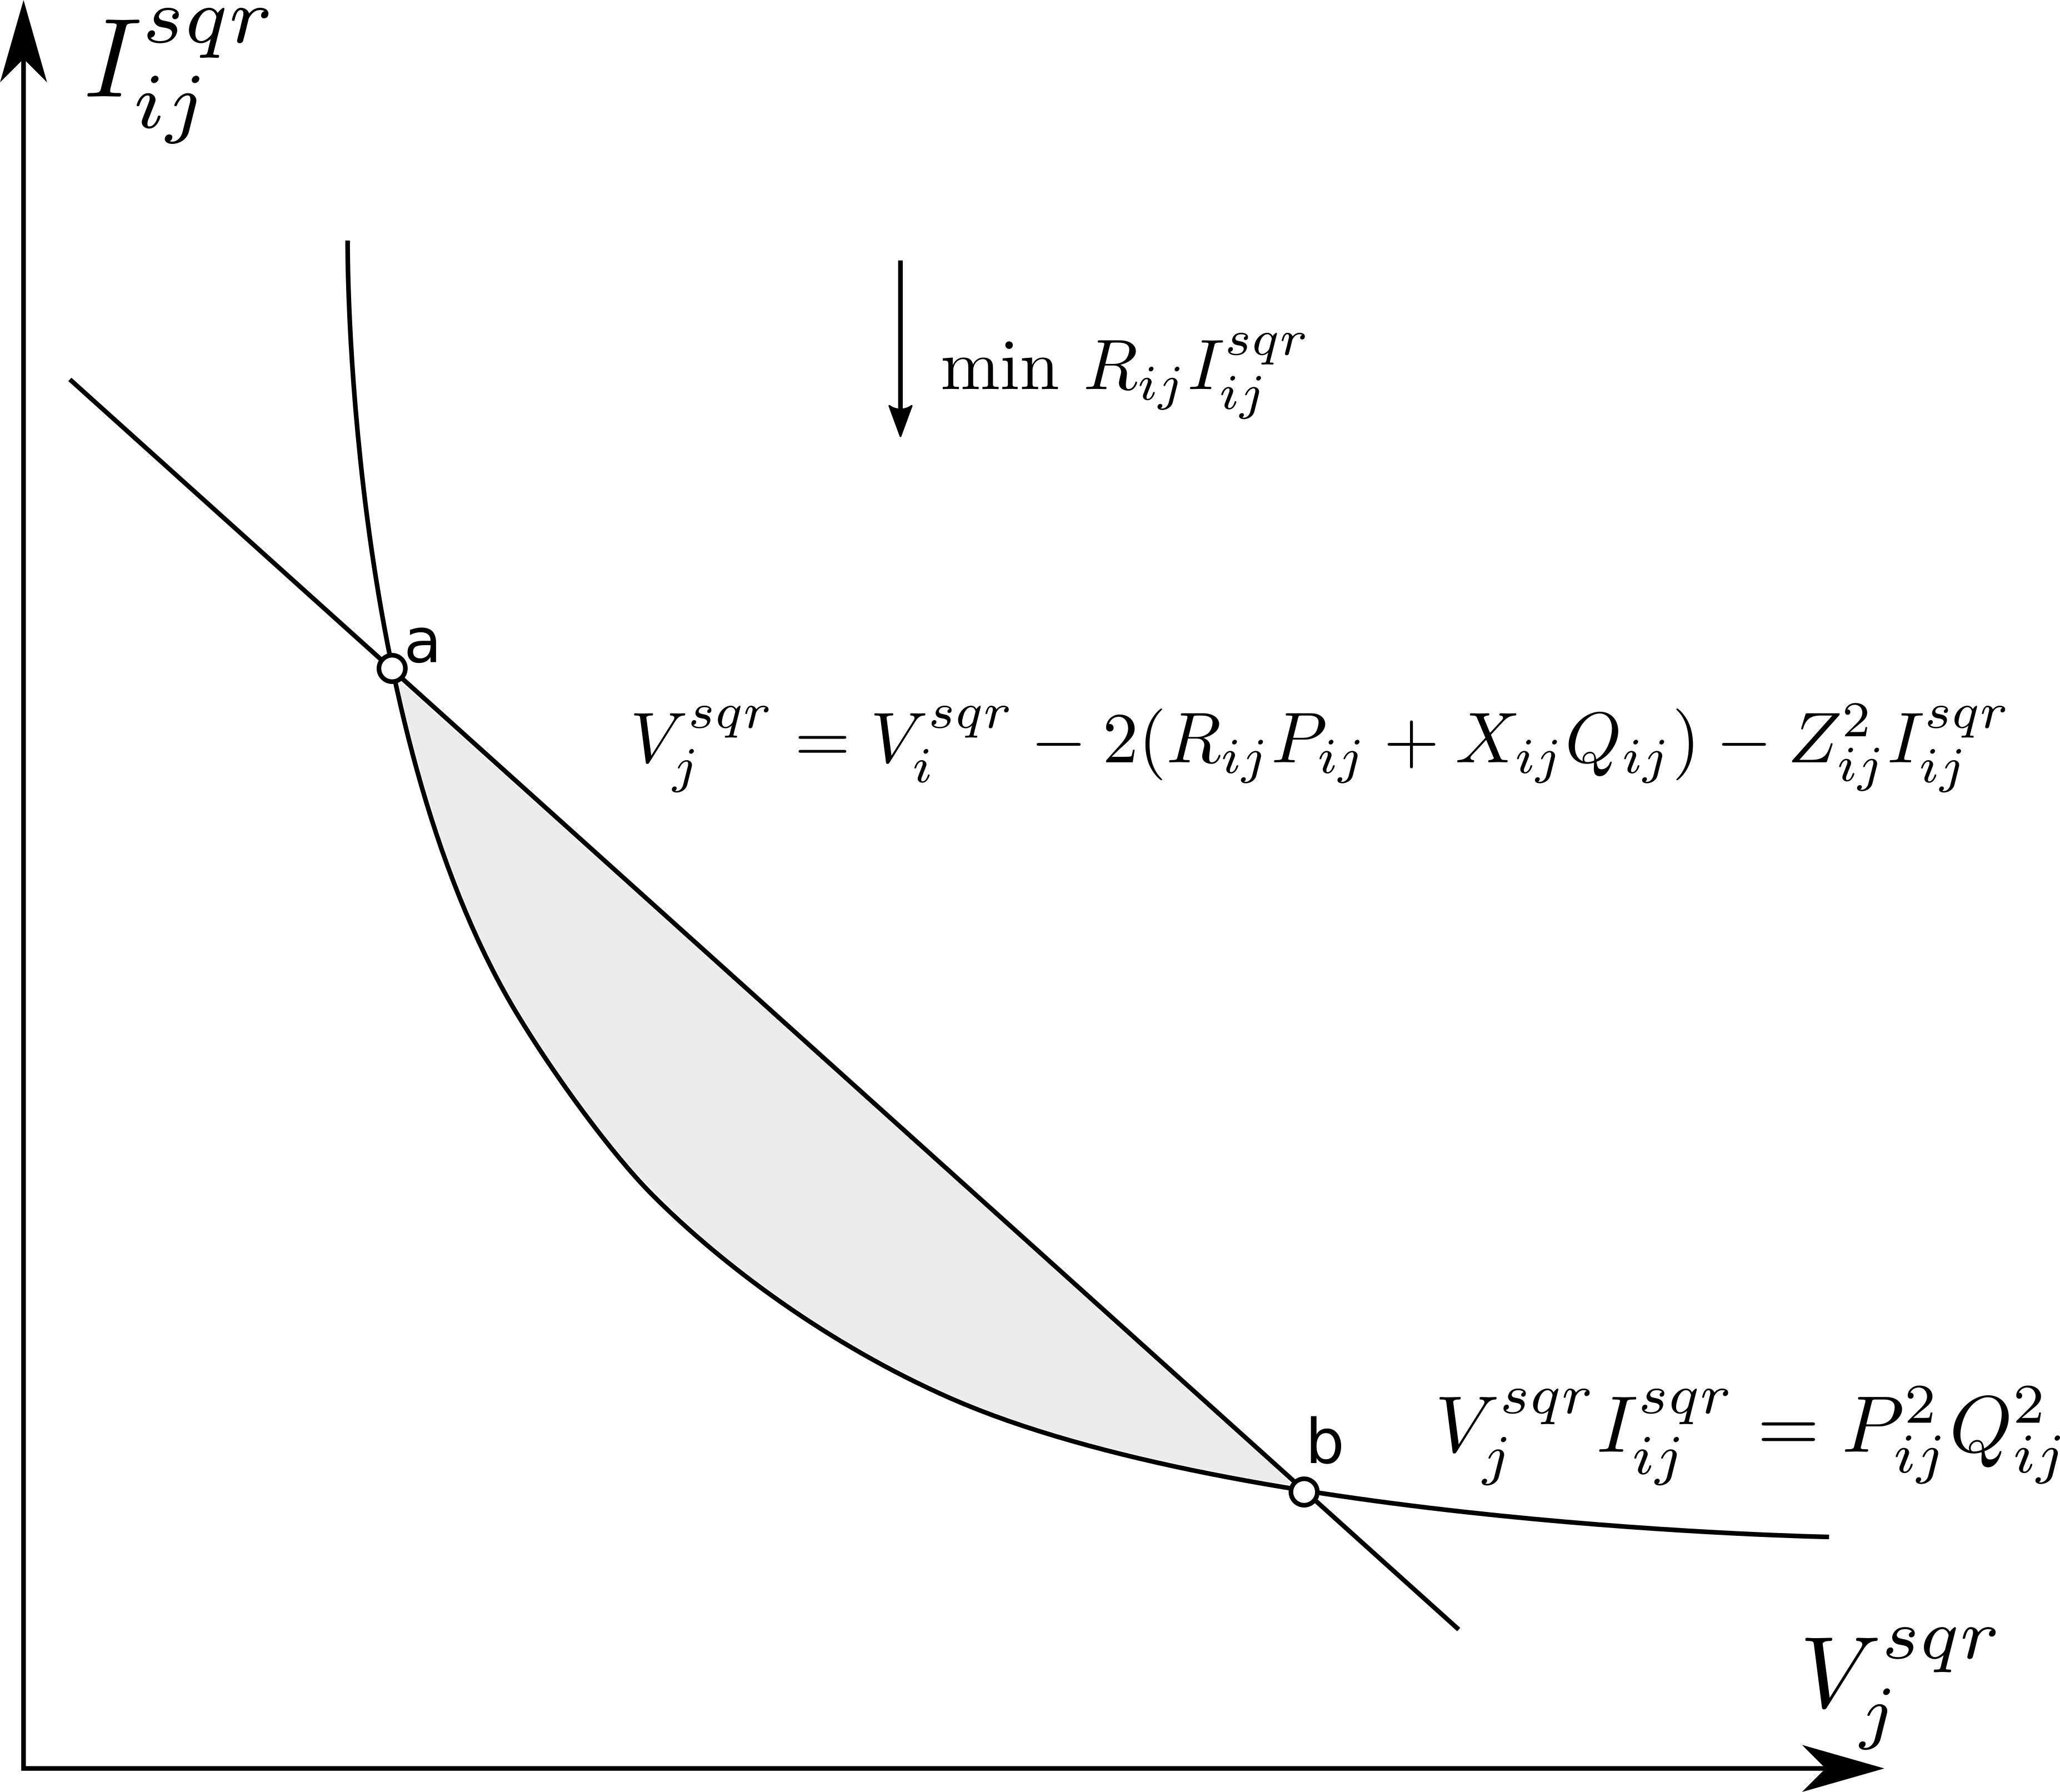
\includegraphics[width =0.6\textwidth]{5_Formulation/pcsoim.png}
    \caption{Representação das restrições~\eqref{eq:pcsoim_power} e \eqref{eq:queda_tensao_restricao} (fonte: \cite{Tatiane2011APLICACAORADIAIS}).}
    \label{fig:pcsoim}
\end{figure}


A região sombreada da figura~\ref{fig:pcsoim} mostra a região factível entre a restrição ``relaxada'' expressa pela equação~\eqref{eq:pcsoim_power} e a restrição~\eqref{eq:queda_tensao_restricao}.
O ponto b mostra a solução para a função objetivo linear.

Dessa forma o problema de PCSOIM pode ser descrito através das expressões:

%Colocar as paradas aqui

\begin{tcolorbox}[breakable,pad at break*=1mm,colback=white!10,title =\textbf{Problema de PCSOIM para RSD}]

\begin{equation}\label{eq:pcsoim}
\left.
    \begin{tabular}{ll}
    & Min ~\eqref{eq:PNLIM_funcobj}\\
    Sujeito a: &\eqref{eq:PNLIM_fluxoP} - \eqref{eq:PNLIM_voltage}, \eqref{eq:PNLIM_voltagekeys} - \eqref{eq:PNLIM_currentlim} \textbf{(Equações já propostas para RSD)}\\
    & \textbf{Relaxamento da equação~\eqref{eq:PNLIM_power}}\\
    & $V_{j}^{sqr}I_{ij}^{sqr} \geq P_{ij}^{2} + Q_{ij}^{2} \qquad ij\in\Omega_{l}$\\
    & \textbf{(Definição de variáveis binárias)}\\
    & $w_{ij}\in\{0,1\}\qquad\forall ij\in\Omega_{l}$
    \end{tabular}
\right \}
\end{equation} 
\end{tcolorbox}
